	\chapter{Deep Learning}
	\resetquestioncounter{}
	\begin{qanda}
		\begin{question}
What is a Neural Network?
		\end{question}
		\begin{answer}
Neural Networks replicate the way humans learn, inspired by how the neurons in our brains fire, only much simpler.

The most common Neural Networks consist of three network layers:
	\begin{bulletedlist}
		\item An input layer
		\item A hidden layer (this is the most important layer where feature extraction takes place, and adjustments are made to train faster and function better).
		\item An output layer
	\end{bulletedlist}
 Each sheet contains neurons called ``nodes,'' performing various operations. Neural Networks are used in deep learning algorithms like CNN, RNN, GAN, etc.
		\end{answer}
	\end{qanda}


	\begin{qanda}
		\begin{question}
			What Are Hyperparameters?
		\end{question}
		\begin{answer}
With neural networks, you're usually working with hyperparameters once the data is formatted correctly. A hyperparameter is a parameter whose value is set before the learning process begins. It determines how a network is trained and the structure of the network (such as the number of hidden units, the learning rate, epochs, etc.).
		\end{answer}
	\end{qanda}


	\begin{qanda}
		\begin{question}
How to install TensorFlow 2.0 on Windows?
		\end{question}
		\begin{answer}
Open the Anaconda prompt and run the following code
\textcode{pip install tensorflow==2.8.0 --user}

Open the jupyter notebook, and refresh the page. Now, check the version of the TensorFlow by importing it with the following code in the jupyter notebook.

\textcode{import tensorflow as tf}
\textcode{print(tf.\_\_version\_\_)}
		\end{answer}
	\end{qanda}


	\begin{qanda}
		\begin{question}
How to install TensorFlow 2.0 on Mac?
		\end{question}
		\begin{answer}
Open your jupyter notebook in your Mac
To install TensorFlow, use the below command and run
\textcode{pip install tensorflow==2.8.0}

Open the jupyter notebook, and refresh the page. Now, check the version of the TensorFlow by importing it with the following code in the jupyter notebook.
\textcode{import tensorflow as tf}
\textcode{print(tf.\_\_version\_\_)}
		\end{answer}
	\end{qanda}


	\begin{qanda}
		\begin{question}
How to resolve the following error while importing Tensorflow?
		\end{question}
		\begin{answer}
``ImportError: DLL load failed: The specified module could not be found''

You can solve this error by downloading and installing visual studio 2015-2019 x86 and x64 from here (Links to an external site.)

Another solution is downgrading the TensorFlow version to 2.0:

\textcode{pip install tensorflow==2.0}

		\end{answer}
	\end{qanda}


	\begin{qanda}
		\begin{question}
What are activation functions?
		\end{question}
		\begin{answer}
In simple terms, an artificial neuron calculates the `weighted sum' of its inputs and adds a bias.

Now the value of net input can be anything from -8 to +8. The neuron doesn't really know how to bound to value and thus is not able to decide the firing pattern. Thus the activation function is an important part of an artificial neural network. They basically decide whether a neuron should be activated or not. Thus it bounds the value of the net input.  The activation function is a non-linear transformation that we do over the input before sending it to the next layer of neurons or finalizing it as output.
		\end{answer}
	\end{qanda}


	\begin{qanda}
		\begin{question}
What Are the Softmax and ReLU Functions?
		\end{question}
		\begin{answer}
Softmax is an activation function that generates the output between zero and one. It divides each output, such that the total sum of the outputs is equal to one. Softmax is often used for output layers.

ReLU (or Rectified Linear Unit) is the most widely used activation function. It gives an output of X if X is positive and zeroes otherwise. ReLU is often used for hidden layers.
		\end{answer}
	\end{qanda}

	\begin{qanda}
		\begin{question}
What Do You Understand by Backpropagation?
		\end{question}
		\begin{answer}
Backpropagation is a technique to improve the performance of the network. It back-propagates the error and updates the weights to reduce the error.
		\end{answer}
	\end{qanda}

	\begin{qanda}
		\begin{question}
What Is Gradient Descent?
		\end{question}
		\begin{answer}
Gradient Descent is an optimal algorithm to minimize the cost function or to minimize an error. The aim is to find the local-global minima of a function. This determines the direction the model should take to reduce the error.
		\end{answer}
	\end{qanda}

	\section{Using File with Google Colab}

Open your drive, create a folder, and upload the data set and notebook in the folder as shown in the below image.

	\begin{figure}[h]
		\centering
		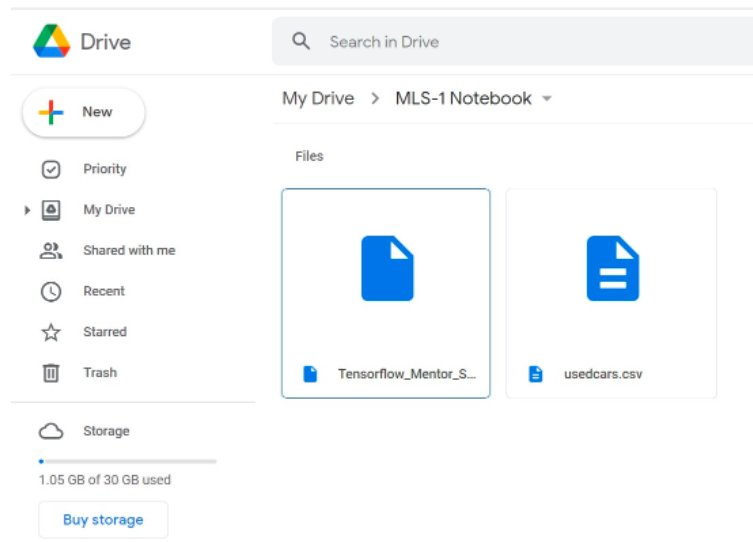
\includegraphics[height=2.0in]{googlecolab1}
		\caption{.}
		\label{fig:googlecolab1}
	\end{figure}

Now right-click on the notebook to open the notebook in Google Colab as shown below.

	\begin{figure}[h]
		\centering
		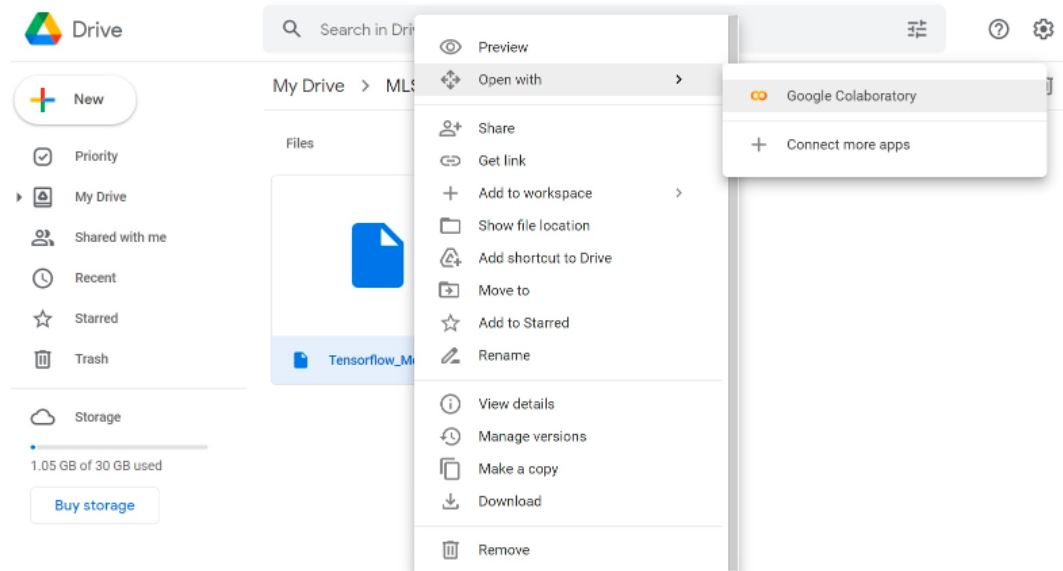
\includegraphics[height=2.0in]{googlecolab2}
		\caption{.}
		\label{fig:googlecolab2}
	\end{figure}

After opening the notebook, you will see the notebook on the Google Colab platform.

	\begin{figure}[h]
		\centering
		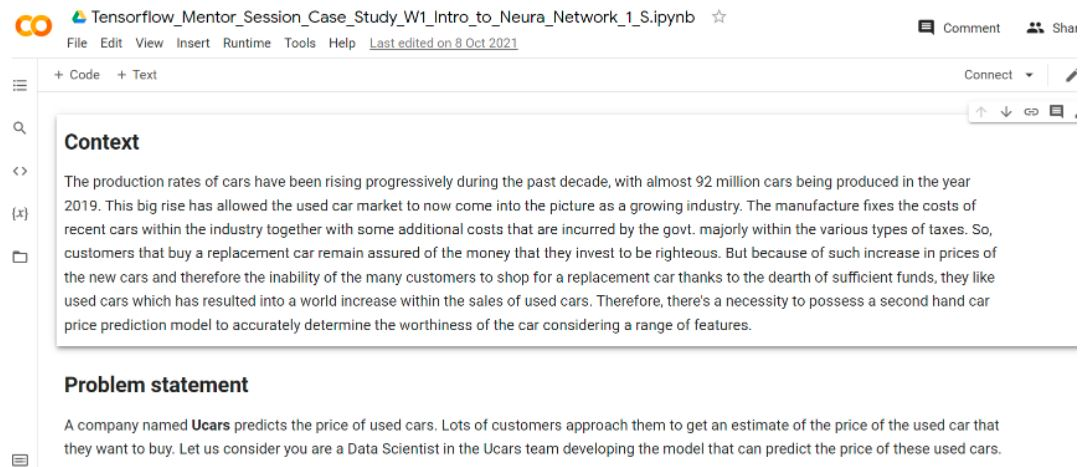
\includegraphics[height=2.0in]{googlecolab3}
		\caption{.}
		\label{fig:googlecolab3}
	\end{figure}

Mount the drive to colab by running the code as shown in the below image.

 	\begin{figure}[h]
		\centering
		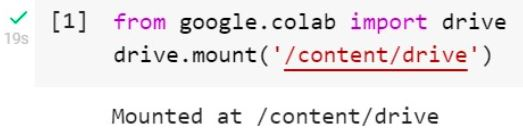
\includegraphics[height=0.75in]{googlecolab4}
		\caption{.}
		\label{fig:googlecolab4}
	\end{figure}

Code:

from google.colab import drive
drive.mount('/content/drive')

Now you can click on the folder icon on the left panel and then go to the folder where you have stored your data set. Then copy the path of the data set by clicking on the three dots beside the data set and click copy and paste it inside the code as shown below.

 	\begin{figure}[h]
		\centering
		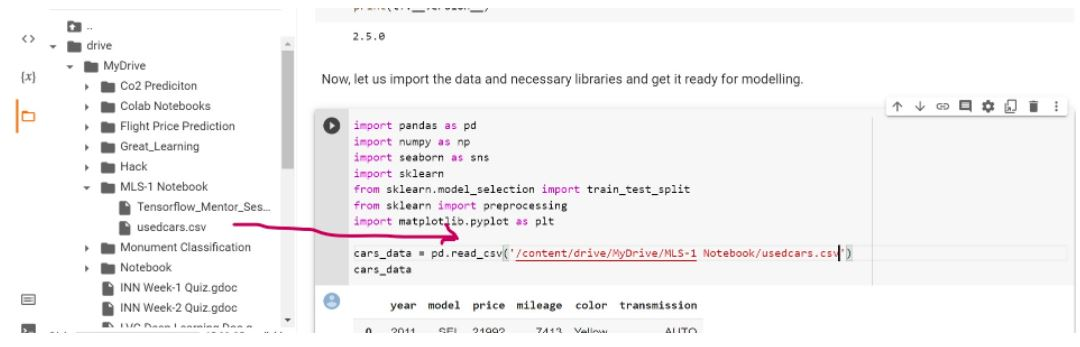
\includegraphics[height=1.75in]{googlecolab5}
		\caption{.}
		\label{fig:googlecolab5}
	\end{figure}


	\section{History}

	\begin{bulletedlist}
		\item Deep Neural Network is an Artificial Neural Network with more than one hidden layer.
		\item An artificial Neural Network (ANN) is a model that employs a collection of artificial neurons to extract the patterns in the data that represent the relationship between independent and dependent variables.
		\item Artificial Neurons are based on the observed behavior of neurons in biological brains. A collection of artificial neurons mimic the behavior of biological neural networks.
		\item Just as brain uses a network of interconnected neurons to parallelize the processing of input signals to trigger a response, ANN also make use of interconnected neurons to work in parallel on input signals and give an output.
		\item In the initial days of the journey towards modern Deep Neural Networks, the research in artificial neuron and ANN were closely tied to the research in
neurology. The research in ANN borrowed ideas such as thresholds, linear summation, neuron firing or not etc from Neurology.
		\item However, the two fields today are de-linked and one does not need to know anything about biological neurons to work on ANN / DNN.
	\end{bulletedlist}
